\documentclass[bachelor, och, pract_otchet]{SCWorks}
% параметр - тип обучения - одно из значений:
%    spec     - специальность
%    bachelor - бакалавриат (по умолчанию)
%    master   - магистратура
% параметр - форма обучения - одно из значений:
%    och   - очное (по умолчанию)
%    zaoch - заочное
% параметр - тип работы - одно из значений:
%    referat    - реферат
%    coursework - курсовая работа (по умолчанию)
%    diploma    - дипломная работа
%    pract      - отчет по практике
% параметр - включение шрифта
%    times    - включение шрифта Times New Roman (если установлен)
%               по умолчанию выключен
\usepackage{subfigure}
\usepackage{tikz,pgfplots}
\pgfplotsset{compat=1.5}
\usepackage{float}

%\usepackage{titlesec}
\setcounter{secnumdepth}{4}
%\titleformat{\paragraph}
%{\normalfont\normalsize}{\theparagraph}{1em}{}
%\titlespacing*{\paragraph}
%{35.5pt}{3.25ex plus 1ex minus .2ex}{1.5ex plus .2ex}

\titleformat{\paragraph}[block]
{\hspace{1.25cm}\normalfont}
{\theparagraph}{1ex}{}
\titlespacing{\paragraph}
{0cm}{2ex plus 1ex minus .2ex}{.4ex plus.2ex}

% --------------------------------------------------------------------------%
\usepackage[T2A]{fontenc}
\usepackage[utf8]{inputenc}
\usepackage{graphicx}
\graphicspath{ {./img/} }
\usepackage{tempora}

\usepackage[sort,compress]{cite}
\usepackage{amsmath}
\usepackage{amssymb}
\usepackage{amsthm}
\usepackage{fancyvrb}
\usepackage{listings}
\usepackage{listingsutf8}
\usepackage{longtable}
\usepackage{array}
\usepackage[english,russian]{babel}

\usepackage[colorlinks=true, linkcolor=black]{hyperref}
\usepackage{url}

\usepackage{underscore}
\usepackage{setspace}
\usepackage{indentfirst} 
\usepackage{mathtools}
\usepackage{amsfonts}
\usepackage{enumitem}
\usepackage{tikz}

\usepackage{minted}
\setminted[python3]{style=bw, linenos, breaklines=true, fontsize=\footnotesize}

\newcommand{\eqdef}{\stackrel {\rm def}{=}}
\newcommand{\specialcell}[2][c]{%
\begin{tabular}[#1]{@{}c@{}}#2\end{tabular}}

\renewcommand\theFancyVerbLine{\small\arabic{FancyVerbLine}}

\newtheorem{lem}{Лемма}

\begin{document}

% Кафедра (в родительном падеже)
\chair{теоретических основ компьютерной безопасности и криптографии}

% Тема работы
\title{Нейронные сети}

% Курс
\course{5}

% Группа
\group{531}

% Факультет (в родительном падеже) (по умолчанию "факультета КНиИТ")
\department{факультета КНиИТ}

% Специальность/направление код - наименование
%\napravlenie{09.03.04 "--- Программная инженерия}
%\napravlenie{010500 "--- Математическое обеспечение и администрирование информационных систем}
%\napravlenie{230100 "--- Информатика и вычислительная техника}
%\napravlenie{231000 "--- Программная инженерия}
\napravlenie{10.05.01 "--- Компьютерная безопасность}

% Для студентки. Для работы студента следующая команда не нужна.
% \studenttitle{Студентки}

% Фамилия, имя, отчество в родительном падеже
\author{Стаина Романа Игоревича}

% Заведующий кафедрой
\chtitle{} % степень, звание
\chname{}

%Научный руководитель (для реферата преподаватель проверяющий работу)
\satitle{доцент} %должность, степень, звание
\saname{И.~И.~Слеповичев}

% Руководитель практики от организации (только для практики,
% для остальных типов работ не используется)
% \patitle{к.ф.-м.н.}
% \paname{С.~В.~Миронов}

% Семестр (только для практики, для остальных
% типов работ не используется)
%\term{8}

% Наименование практики (только для практики, для остальных
% типов работ не используется)
%\practtype{преддипломная}

% Продолжительность практики (количество недель) (только для практики,
% для остальных типов работ не используется)
%\duration{4}

% Даты начала и окончания практики (только для практики, для остальных
% типов работ не используется)
%\practStart{30.04.2019}
%\practFinish{27.05.2019}

% Год выполнения отчета
\date{2023}

\maketitle

% Включение нумерации рисунков, формул и таблиц по разделам
% (по умолчанию - нумерация сквозная)
% (допускается оба вида нумерации)
% \secNumbering

%-------------------------------------------------------------------------------------------

% \begin{minted}[fontsize=\small]{MySQL}
% \end{minted}

% \begin{figure}[H]
%     \centering
%     \includegraphics[width=0.999\textwidth]{img/}
%     \caption{}
%     \label{easy_hack}
% \end{figure}

\tableofcontents

\section{Создание ориентированного графа}
\subsection{Описание задачи}
\subsubsection{Вход} 
Текстовый файл с описанием графа в виде списка дуг
\[ (a_1, b_1, n_1), (a_2, b_2, n_2), \dots, (a_k, b_k, n_k) \]
где $a_i$ -- начальная вершина дуги $i$, $b_i$ -- конечная вершина дуги $i$,
$n_i$ -- порядковый номер в списке всех заходящих в вершину $b_i$ дуг.

\subsubsection{Выход}
\begin{enumerate}
  \item Ориентированный граф с именованными вершинами и линейно упорядоченными дугами 
  (в соответствии с порядком из текстового файла).
  \item Сообщение об ошибке в формате файла, если ошибка присутствует.
\end{enumerate}

\subsection{Примеры исполнения}
\begin{figure}[H]
    \centering
    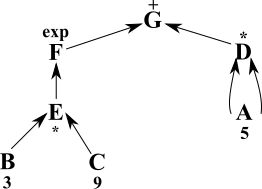
\includegraphics[width=0.4\textwidth]{img/btest1.png}
    \caption{Пример графа}
    \label{1}
\end{figure}

Граф на рисунке \ref{1} задаётся в виде
\[ (A, D, 1), (A, D, 2), (B, E, 1), (C, E, 2), (D, G, 1), (E, F, 1), (F, G, 2) \]

В результате программа вернёт сериализованную структуру графа в формате XML
\begin{minted}[fontsize=\footnotesize]{XML}
  <graph>
  <vertex>A</vertex>
  <vertex>B</vertex>
  <vertex>C</vertex>
  <vertex>D</vertex>
  <vertex>E</vertex>
  <vertex>F</vertex>
  <vertex>G</vertex>
  <arc>
    <from>A</from>
    <to>D</to>
    <order>1</order>
  </arc>
  <arc>
    <from>B</from>
    <to>E</to>
    <order>1</order>
  </arc>
  <arc>
    <from>D</from>
    <to>G</to>
    <order>1</order>
  </arc>
  <arc>
    <from>E</from>
    <to>F</to>
    <order>1</order>
  </arc>
  <arc>
    <from>A</from>
    <to>D</to>
    <order>2</order>
  </arc>
  <arc>
    <from>C</from>
    <to>E</to>
    <order>2</order>
  </arc>
  <arc>
    <from>F</from>
    <to>G</to>
    <order>2</order>
  </arc>
</graph>
\end{minted}

\begin{figure}[H]
  \centering
  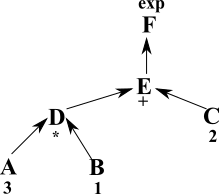
\includegraphics[width=0.4\textwidth]{img/btest2.png}
  \caption{Пример графа}
  \label{2}
\end{figure}

Граф на рисунке \ref{2} задаётся в виде
\[ (A, D, 1), (B, D, 2), (D, E, 1), (C, E, 2), (E, F, 1) \]

В результате программа вернёт сериализованную структуру графа в формате XML
\begin{minted}[fontsize=\footnotesize]{XML}
  <graph>
  <vertex>A</vertex>
  <vertex>B</vertex>
  <vertex>C</vertex>
  <vertex>D</vertex>
  <vertex>E</vertex>
  <vertex>F</vertex>
  <arc>
    <from>A</from>
    <to>D</to>
    <order>1</order>
  </arc>
  <arc>
    <from>D</from>
    <to>E</to>
    <order>1</order>
  </arc>
  <arc>
    <from>E</from>
    <to>F</to>
    <order>1</order>
  </arc>
  <arc>
    <from>B</from>
    <to>D</to>
    <order>2</order>
  </arc>
  <arc>
    <from>C</from>
    <to>E</to>
    <order>2</order>
  </arc>
</graph>
\end{minted}

\section{Создание функции по графу}
\subsection{Описание задачи}
\subsubsection{Вход}
Ориентированный граф с именованными вершинами как описано в задании 1.

\subsubsection{Выход}
Линейное представление функции, реализуемой графом в префиксной скобочной записи:
\[ A_1(B_1(C_1(\dots), \dots, C_m(\dots)), \dots, B_n(\dots)) \]

Способ проверки результата:
\begin{enumerate}
  \item выгрузка в текстовый файл результата преобразования графа в имя функции;
  \item сообщение о наличии циклов в графе, если они присутствуют.
\end{enumerate}

\subsection{Описание работы программы}
Циклы в графе обнаруживаются при помощи алгоритма \textbf{DFS}.

Далее для каждой вершины сохраняется список её родителей и детей, находится корневая вершина -- вершина без детей.
Затем от корневой вершины вызывается рекурсивная функция:
\begin{minted}[fontsize=\small]{python}
  def make_func(v, vs):
    parents = [make_func(c, vs) for c in v.parents]
    return f'{v.name}({", ".join(parents)})'
\end{minted}
Эта функция и создаёт функцию по графу в префиксной скобочной записи.

\subsection{Примеры исполнения}
По графу на рисунке \ref{1} функция будет иметь вид:
\[ G(D(A(), A()), F(E(B(), C()))) \]

По графу на рисунке \ref{2} функция будет иметь вид:
\[ F(E(D(A(), B()), C())) \]

\section{Вычисление значения функции на графе}
\subsection{Описание задачи}
\subsubsection{Вход}
\begin{enumerate}
  \item Текстовый файл с описанием графа в виде списка дуг.
  \item Текстовый файл соответствий арифметических операций именам вершин:
  \begin{itemize}
    \item $a_1$: операция $1$,
    \item \dots,
    \item $a_n$: операция $n$.
  \end{itemize}
  где $a_i$ -- имя $i$-й вершины, операция $i$ -- символ операции, соответствующий вершине $a_i$.
\end{enumerate}

Допустимы следующие символы операций: 
\begin{itemize}
  \item + -- cумма значений,
  \item * --  произведение значений,
  \item exp -- экспонирование входного значения,
  \item число -- любая числовая константа.		
\end{itemize}

\subsubsection{Выход}
Значение функции, построенной по графу 1) и файлу 2). 

Способ проверки результата: результат вычисления, выведенный в файл.

\subsection{Описание работы программы}
Для каждой вершины определяется либо её числовое значение, либо операция и проверяется,
что число аргументов, то есть число родителей соответствует операции. 
У вершины с числовым значением не должно быть родителей.

Затем от корневой вершины вызывается рекурсивная функция вычисления значения функции графа:
\begin{minted}[fontsize=\small]{python}
def evaluate(v):
    if v.operation is None:
        return v.value

    if v.operation == '+':
        result = 0
        for p in v.parents:
            result += evaluate(p)
        return result

    if v.operation == '*':
        result = 1
        for p in v.parents:
            result *= evaluate(p)
        return result

    if v.operation == 'exp':
        return exp(evaluate(v.parents[0]))
\end{minted}

\subsection{Примеры исполнения}
На рисунках \ref{1} и \ref{2} подписаны заданные операции. Для первого результат будет --
532048240626.7986, а для второго -- 1096.6331584284585.

\section{Построение многослойной нейронной сети}
\subsection{Описание задачи}
\subsubsection{Вход}
\begin{enumerate}
  \item Текстовый файл с набором матриц весов межнейронных связей.
  \item Текстовый файл с входным вектором.
\end{enumerate}

\subsubsection{Выход}
\begin{enumerate}
  \item Файл с выходным вектором – результатом вычислений НС.
  \item Сообщение об ошибке, если в формате входного вектора или файла описания НС допущена ошибка.
\end{enumerate}

\subsection{Описание работы программы}
Выход каждого нейрона в слое вычисляется следующим образом.
Сначала вычисляется неактивированное состояние $Y = W \cdot X$, где
$W$ -- матрица весовых коэффициентов слоя,
$X$ -- входной вектор. Затем $Y$ передаётся в функцию активации,
в частности, сигмоиду:
\[ f(x) = \displaystyle\frac{1}{1 + e^{-x}} \]

Далее активированные значения $y_i$ из $Y$ передаются на следующий
слой в качестве входного вектора. Полученные выходные значения
на последнем слое и будут результатом вычисления нейронной сети.

\subsection{Пример исполнения}
На вход подаются матрицы весов:
\begin{table}[H]
  \begin{tabular}{|l|l|l|}
  \hline
  0.1 & 0.5 & 0.9 \\ \hline
  0.2 & 0.4 & 0.8 \\ \hline
  0.1 & 0.1 & 0.1 \\ \hline
  0.3 & 0.6 & 0.9 \\ \hline
  0.0 & 0.5 & 1.0 \\ \hline
  \end{tabular}
  \caption{Матрица весов первого слоя}
\end{table}
В 1 слое 5 нейронов с 3 входами.

\begin{table}[H]
  \begin{tabular}{|l|l|l|l|l|}
  \hline
  0.1 & 0.2 & 0.3 & 0.4 & 0.5 \\ \hline
  0.15 & 0.25 & 0.35 & 0.45 & 0.55 \\ \hline
  0.9 & 0.8 & 0.7 & 0.6 & 0.5 \\ \hline
  \end{tabular}
  \caption{Матрица весов второго слоя}
\end{table}
Во 2 слое 3 нейрона с 5 входами. 

Входной вектор:
\[ X = [2.47, 1.2, 9.6] \]

Выходной вектор:
\[ Y = [0.8079936459041838, 0.8424440351919794, 0.9662026046584478] \]

\section{Реализация метода обратного распространения ошибки для многослойной НС}
\subsection{Описание задачи}
\subsubsection{Вход}
\begin{enumerate}
  \item Текстовый файл с описанием НС.
  \item Текстовый файл с обучающей выборкой.
  \item Текстовый файл с параметрами обучения 
  (скорость обучения, погрешность, колличество итераций).
\end{enumerate}

\subsubsection{Выход}
\begin{enumerate}
  \item Текстовый файл с историей итераций обучения методом обратного 
  распространения ошибки.
  \item Результирующий вектор, полученный после обучения НС.
\end{enumerate}

\subsection{Описание работы программы}
В предыдущем задании НС выдаёт <<случайные>> значения, зависящие
от заданных матриц весов и входного вектора. Однако требуется, чтобы
ответы сети удовлетворяли поставленной задаче, поэтому её необходимо обучить.

\subsubsection{Обратное распространение ошибки}
Для обучения будет использоваться обратное распространение ошибки, 
работающее по следующему алгоритму:
\begin{enumerate}
  \item Подать на вход сети обучающий пример (один входной вектор).
  \item Распространить сигнал по сети вперёд (получить выход сети).
  \item Вычислить ошибку (разница получившегося и ожидаемого векторов).
  \item Распространить ошибку на предыдущие слои.
  \item Обновить весовые коэффициенты для уменьшения ошибки.
\end{enumerate}
Алгоритм останавливается, когда будет достигнута заданная точность 
или будет исчерпано число итераций.

Для каждого слоя сохраняется его вход $x$, выход $z$ и производная функции $df$ активации, а
так же вектор дельт.

В качестве функции оценки сети $E(W)$ используется среднее квадратичное отклонение
\[ E = \frac{1}{2} \cdot \sum(y_{1i} - y_{2i})^2. \]
Чтобы найти значение ошибки E, нужно найти сумму квадратов разности значений вектора, 
который выдала сеть в качестве ответа, и вектора, который ожидается при обучении. 

Также нужно найти дельту для каждого слоя, 
причём для последнего слоя она будет равна вектору разности
полученного и ожидаемого векторов, умноженному (покомпонентно) 
на вектор значений производных последнего слоя: 
\[ \delta_{last} = (z_{last} - d) \cdot f'_{last}, \]
где $z_{last}$ -- выход последнего слоя сети, $d$ -- ожидаемый вектор сети,
$f`_last$ -- вектор значений производной функции активации последнего слоя.

Чтобы найти дельты предыдущих слоёв:
\[ \delta_{k - 1} = W_k^T \cdot \delta_k \cdot f'_k, \]
где $W_k^T$ -- транспонированная матрица весов $k$-го слоя.

\subsubsection{Изменение весов}
Для того, чтобы уменьшить ошибку сети нужно изменить весовые коэффициенты каждого слоя.
Для этого используется метод градиентного спуска.
Градиент по весам равен перемножению входного вектора и вектора дельт.
Поэтому, чтобы обновить весовые коэффициенты и уменьшить тем самым ошибку
сети нужно вычесть из матрицы весов результат перемножения дельт и входных векторов, 
умноженный на скорость обучения.
\[ W_{k} = W_k - \alpha \cdot \delta_k \cdot X_k, \]
где $W_k$ -- матрица весов $k$-го слоя, $\alpha$ -- скорость обучения, 
$\delta_k$ - дельта $k$-го слоя, $X_k$ -- входной вектор $k$-го слоя.

\subsection{Примеры исполнения}
Первый тест представляет собой обучение НС функции xor. 
В первом слое два нейрона с 2 входами, во втором слое один нейрон с 1 входом.
В приложении Е можно увидеть входные файлы и выдержку из истории обучения.
В результате обучения НС выдала такой результат:
\begin{minted}[fontsize=\footnotesize]{text}
  X: [0 0], Y: [0.], out: [0.07254825]
  X: [0 1], Y: [1.], out: [0.87228817]
  X: [1 0], Y: [1.], out: [0.87094845]
  X: [1 1], Y: [0.], out: [0.13987849]
\end{minted}

Были получены значения, близкие к истинным. 

Во втором тесте НС должна угадать, какое число изображено на табло.
\begin{table}[H]
  \begin{tabular}{|l|l|l|}
  \hline
  1   & 2   & 3 \\ \hline
  4   & 5   & 6 \\ \hline
  7   & 8   & 9 \\ \hline
  10  & 11  & 12 \\ \hline
  13  & 14  & 15 \\ \hline
  \end{tabular}
  \caption{Матрица с номерами пикселей}
\end{table}

Например, если загадано число 4, то будут гореть пиксели 1, 3, 4, 6, 7, 8, 9, 12, 15.
В качестве входного вектора задаётся вектор длины 15, где если пиксель с номером $1 \geq i \geq 15$ горит,
то на $i$-м месте стоит 1, иначе 0. То есть число 4 будет иметь вид:
\[ [1, 0, 1, 1, 0, 1, 1, 1, 1, 0, 0, 1, 0, 0, 1] \]
Поскольку используется сигмоидная функция в качестве функции активации, ответы могут принимать значения
от 0 до 1, поэтому эталонными значениями тоже будут числа от 0 до 1. То есть число 4 задаётся в виде 0.4.

В первом слое пять нейронов с 15 входами, во втором три нейрона
с 5 входами и на третьем один нейрон с 3 входами.

В результате обучения НС выдала такой результат:
\begin{minted}[fontsize=\footnotesize]{text}
  X: [1 1 1 1 0 1 1 0 1 1 0 1 1 1 1], Y: [0.], out: [0.00650746]
  X: [0 0 1 0 0 1 0 0 1 0 0 1 0 0 1], Y: [0.1], out: [0.10080306]
  X: [1 1 1 0 0 1 1 1 1 1 0 0 1 1 1], Y: [0.2], out: [0.2023985]
  X: [1 1 1 0 0 1 1 1 1 0 0 1 1 1 1], Y: [0.3], out: [0.30715552]
  X: [1 0 1 0 0 1 1 1 1 0 0 1 0 0 1], Y: [0.4], out: [0.40414067]
  X: [1 1 1 1 0 0 1 1 1 0 0 1 1 1 1], Y: [0.5], out: [0.49959161]
  X: [1 1 1 1 0 0 1 1 1 1 0 1 1 1 1], Y: [0.6], out: [0.59926368]
  X: [1 1 1 0 0 1 0 0 1 0 0 1 0 0 1], Y: [0.7], out: [0.69969015]
  X: [1 1 1 1 0 1 1 1 1 1 0 1 1 1 1], Y: [0.8], out: [0.80022029]
  X: [1 1 1 1 0 1 1 1 1 0 0 1 1 1 1], Y: [0.9], out: [0.90026761]  
\end{minted}

\newpage
\appendix
    \section{Листинг задания 1}
    \inputminted[fontsize=\footnotesize]{python3}{nntask1.py}

    \section{Листинг задания 2}
    \inputminted[fontsize=\footnotesize]{python3}{nntask2.py}

    \section{Листинг задания 3}
    \inputminted[fontsize=\footnotesize]{python3}{nntask3.py}

    \section{Листинг задания 4}
    \inputminted[fontsize=\footnotesize]{python3}{nntask4.py}

    \section{Листинг задания 5}
    \inputminted[fontsize=\footnotesize]{python3}{nntask5.py}

    \section{Тестовые файлы для задания 5}
      \begin{listing}[H]
        \begin{minted}[fontsize=\footnotesize]{text}
          {
            "w1": [[0.45, -0.12], [0.78, 0.13]],
            "w2": [[1.5, -2.3]]
          }
        \end{minted}
        \caption{Матрицы весов для обучения xor}
      \end{listing}

      \begin{listing}[H]
        \begin{minted}[fontsize=\footnotesize]{text}
          {
            "x": [[0, 0], [0, 1], [1, 0], [1, 1]],
            "y": [[0.0], [1.0], [1.0], [0.0]]
          }
        \end{minted}
        \caption{Выборка для обучения xor}
      \end{listing}

      \begin{listing}[H]
        \begin{minted}[fontsize=\footnotesize]{text}
          {
            "iters": 10000,
            "alpha": 0.5,
            "eps": 0.000001
          }
        \end{minted}
        \caption{Параметры для обучения xor}
      \end{listing}

      \begin{listing}[H]
        \begin{minted}[fontsize=\footnotesize]{text}
          1: 0.13899320498724652
          5000: 0.037662754759293815
          10000: 0.008381458044956066
        \end{minted}
        \caption{Выдержка из истории обучения xor}
      \end{listing}

      \begin{listing}[H]
        \begin{minted}[fontsize=\footnotesize]{text}
        {
        "w1": [
                [0.696, 0.282, 0.059, 0.024, 0.275, 0.236, 0.973, 0.378, 
                0.016, 0.717, 0.238, 0.202, 0.309, 0.541, 0.456],
                [0.285, 0.433, 0.259, 0.807, 0.294, 0.794, 0.268, 0.205, 
                0.247, 0.772, 0.300, 0.575, 0.844, 0.578, 0.938],
                [0.454, 0.824, 0.0794, 0.473, 0.946, 0.378, 0.541, 0.167, 
                0.089, 0.019, 0.881, 0.630, 0.083, 0.967, 0.892],
                [0.258, 0.362, 0.31, 0.557, 0.499, 0.967, 0.443, 0.951, 
                0.248, 0.454, 0.894, 0.996, 0.418, 0.997, 0.619],
                [0.399, 0.942, 0.245, 0.769, 0.313, 0.611, 0.34, 0.756, 
                0.03, 0.065, 0.655, 0.832, 0.399, 0.684, 0.815]
              ],
        "w2": [
                [0.231, 0.533, 0.541, 0.409, 0.232],
                [0.479, 0.641, 0.731, 0.159, 0.403],
                [0.525, 0.547, 0.93, 0.698, 0.849]
              ],
        "w3": [
                [0.507, 0.838, 0.672]
              ]
        }
        \end{minted}
        \caption{Матрицы весов для обучения угадыванию числа}
      \end{listing}

      \begin{listing}[H]
        \begin{minted}[fontsize=\footnotesize]{text}
          {
            "x": [
                  [1, 1, 1, 1, 0, 1, 1, 0, 1, 1, 0, 1, 1, 1, 1],
                  [0, 0, 1, 0, 0, 1, 0, 0, 1, 0, 0, 1, 0, 0, 1],
                  [1, 1, 1, 0, 0, 1, 1, 1, 1, 1, 0, 0, 1, 1, 1],
                  [1, 1, 1, 0, 0, 1, 1, 1, 1, 0, 0, 1, 1, 1, 1],
                  [1, 0, 1, 0, 0, 1, 1, 1, 1, 0, 0, 1, 0, 0, 1],
                  [1, 1, 1, 1, 0, 0, 1, 1, 1, 0, 0, 1, 1, 1, 1],
                  [1, 1, 1, 1, 0, 0, 1, 1, 1, 1, 0, 1, 1, 1, 1],
                  [1, 1, 1, 0, 0, 1, 0, 0, 1, 0, 0, 1, 0, 0, 1],
                  [1, 1, 1, 1, 0, 1, 1, 1, 1, 1, 0, 1, 1, 1, 1],
                  [1, 1, 1, 1, 0, 1, 1, 1, 1, 0, 0, 1, 1, 1, 1]
                 ],
            "y": [[0.0], [0.1], [0.2], [0.3], [0.4], [0.5], [0.6], [0.7], [0.8], [0.9]]
          }
        \end{minted}
        \caption{Выборка для обучения угадыванию числа}
      \end{listing}

      \begin{listing}[H]
        \begin{minted}[fontsize=\footnotesize]{text}
          {
            "iters": 25000,
            "alpha": 0.75,
            "eps": 0.000001
          }
        \end{minted}
        \caption{Параметры для обучения угадыванию числа}
      \end{listing}

      \begin{listing}[H]
        \begin{minted}[fontsize=\footnotesize]{text}
          1: 0.1137608520762083
          5000: 0.0005942319497309006
          10000: 0.00030233336286510624
          25000: 2.9506600016289843e-05
          50000: 9.024999353650563e-06
        \end{minted}
        \caption{Выдержка из истории обучения угадыванию числа}
      \end{listing}

\end{document}